\chapter{Del principio de equivalencia a los tensores}

La relatividad general suele abreviarse como RG, aunque rara vez se llama RE a la relatividad especial. La abreviatura importa menos que la decisión de empezar por el principio. La vía más directa es la que siguió Einstein: partir de una observación física que pueda percibirse en un ascensor, llevarla hasta que sus consecuencias sean ineludibles y solo entonces introducir la geometría.

La primera observación es el principio de equivalencia. La gravedad y la aceleración son localmente indistinguibles. La palabra localmente acabará soportando casi todo el peso de esta afirmación. Sin embargo, antes de precisarla, veamos qué permite hacer ya la afirmación sin matices.

\section{El ascensor como transformación de coordenadas}

Los libros de texto suelen sustituir el ascensor de Einstein por una nave espacial. Aquí es preferible el ascensor porque su aceleración nos resulta familiar. Sea \(z\) la altura medida en un sistema de referencia ligado al suelo y \(z'\) la altura medida desde el piso del ascensor. Si el piso está a la altura \(L(t)\), el mismo suceso tiene las coordenadas
\begin{equation}
 z'=z-L(t),\qquad t'=t,\qquad x'=x.
\label{eq:elevator-map}
\end{equation}
La coordenada horizontal no cambia porque el ascensor no se desplaza lateralmente. Al tomar deliberadamente \(t'=t\), dejamos de lado por el momento la relatividad especial.

\begin{classroomqa}
\audiencequestion{¿Cómo puede empezar un curso de relatividad general ignorando la relatividad especial?}
\lecturerresponse{Hay un régimen en el que la gravedad es importante, mientras que todas las velocidades siguen siendo pequeñas comparadas con \(c\). Por tanto, la conexión entre gravedad--aceleración puede aislarse en la mecánica newtoniana y combinarse después con la geometría de Minkowski. Es una elección didáctica, no una afirmación de que la teoría final sea no relativista. \lecturetimestamp{00:05:33}}
\end{classroomqa}

En dos sistemas inerciales, el ascensor se mueve uniformemente:
\begin{equation}
 L(t)=vt,\qquad z'=z-vt.
\label{eq:galilean-elevator}
\end{equation}
Se ha elegido que los orígenes coincidan en \(t=0\). La pizarra mantiene el esquema del ascensor junto a las tres relaciones entre coordenadas, para que los símbolos nunca pierdan su significado físico.

\begin{figure}[H]
\centering
\includegraphics[width=\linewidth]{lecture_01_figure_01.png}
\caption{Coordenadas del ascensor tras particularizar al caso de velocidad uniforme \(L(t)=vt\).}
\par\smallskip
\textit{Marco de la clase: 00:09:10.}
\end{figure}

Consideremos solo la componente vertical de la segunda ley de Newton:
\begin{equation}
 F=m\ddot z.
\label{eq:newton-unprimed}
\end{equation}
La fuerza puede deberse a una cuerda, un campo eléctrico o cualquier otra interacción ordinaria. Al derivar dos veces \eqref{eq:galilean-elevator}, se obtiene
\(\ddot z'=\ddot z\), y, por tanto,
\begin{equation}
 F=m\ddot z'.
\label{eq:newton-primed-inertial}
\end{equation}
La forma de la ley no cambia. Este cálculo elemental pone de manifiesto el contenido operativo de la equivalencia entre sistemas inerciales: una transformación lineal de coordenadas lleva un movimiento uniforme a otro movimiento uniforme.

\begin{figure}[H]
\centering
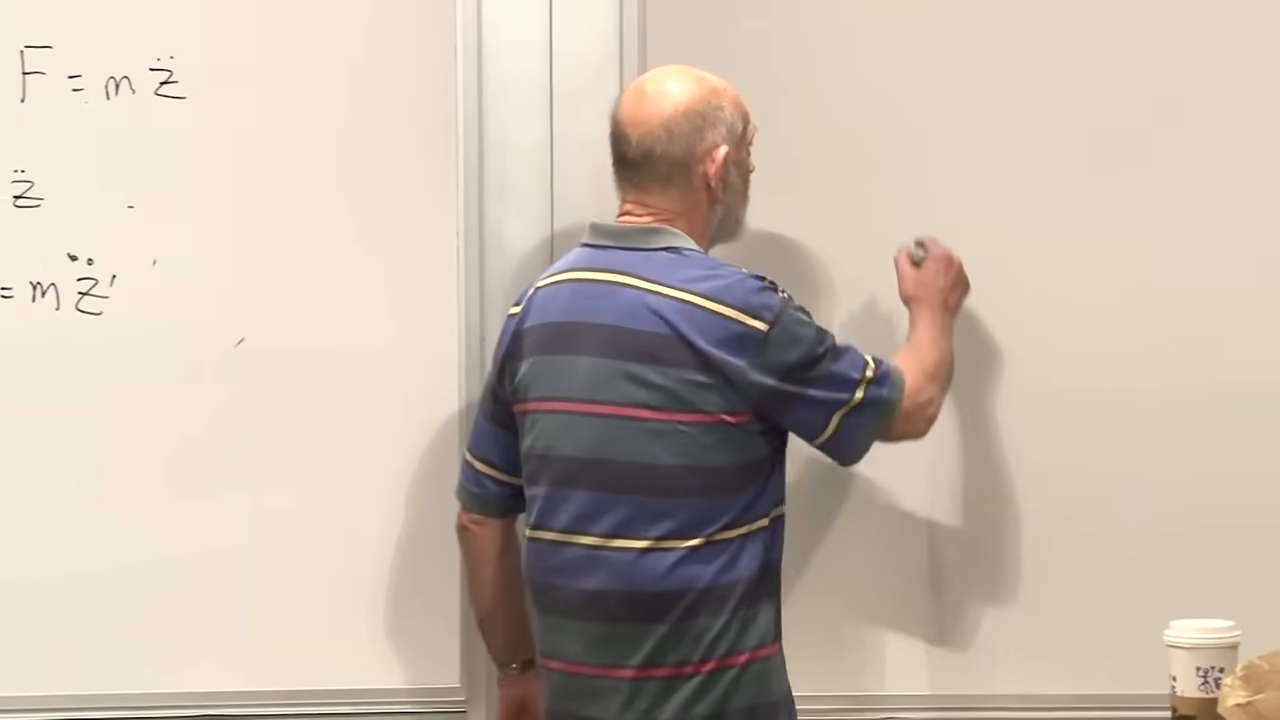
\includegraphics[width=\linewidth]{lecture_01_figure_02.png}
\caption{Ecuación de Newton en dos sistemas de coordenadas que se mueven uniformemente.}
\par\smallskip
\textit{Marco de la clase: 00:11:50.}
\end{figure}

Ahora aceleremos el ascensor hacia arriba con aceleración constante \(g\):
\begin{equation}
 L(t)=\frac12gt^2,\qquad
 \dot L=gt,\qquad
 \ddot L=g.
\end{equation}
La transformación de coordenadas pasa a ser
\begin{equation}
 z'=z-\frac12gt^2,
\qquad
 \ddot z'=\ddot z-g.
\label{eq:accelerated-map}
\end{equation}
Al sustituirla en la ley de Newton, se obtiene
\begin{equation}
 F=m(\ddot z'+g),
\qquad
 m\ddot z'=F-mg.
\label{eq:fictitious-gravity}
\end{equation}
La derivación incluye una comprobación de signos útil en directo: \(+mg\) aparece primero en el lado de la aceleración y se convierte en \(-mg\) solo al pasar al lado de las fuerzas. En el sistema cuyo piso acelera hacia arriba, el sentido final es hacia abajo.

\begin{figure}[H]
\centering
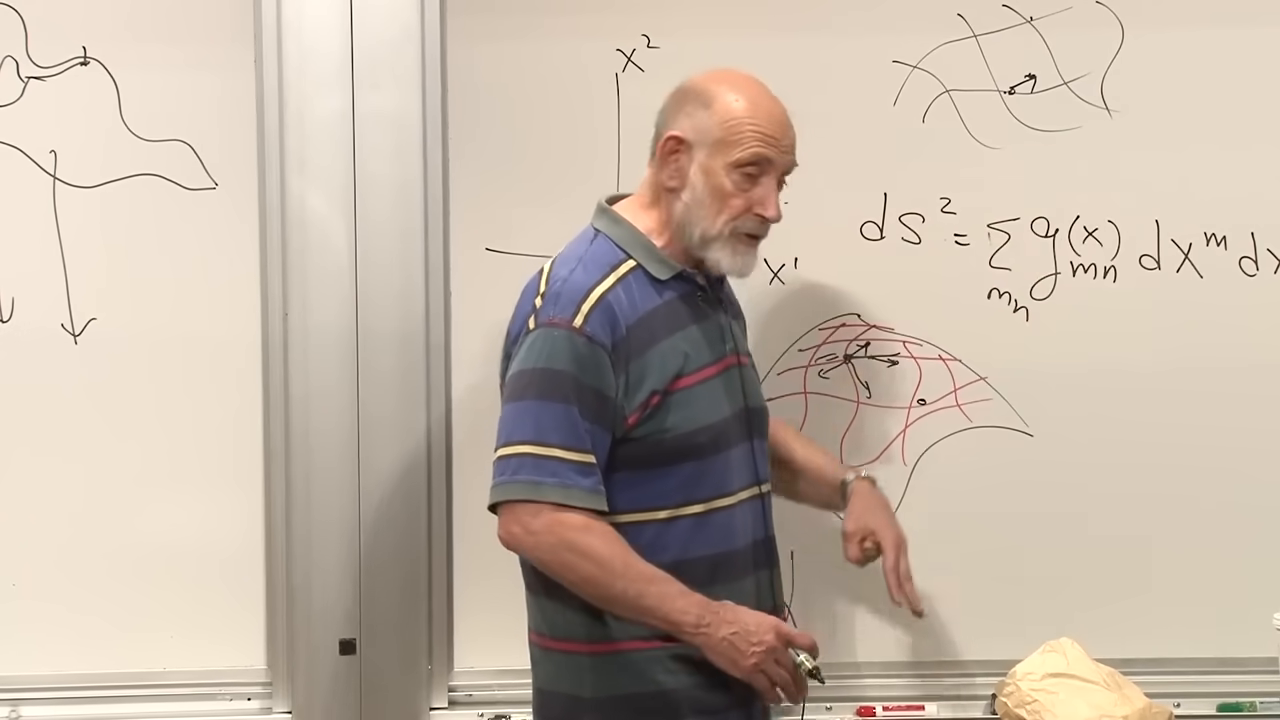
\includegraphics[width=\linewidth]{lecture_01_figure_03.png}
\caption{La transformación acelerada y la fuerza ficticia resultante \(-mg\).}
\par\smallskip
\textit{Marco de la clase: 00:15:35.}
\end{figure}

El nuevo término parece gravitatorio por una razón precisa: es proporcional a la masa. Como la respuesta inercial también es proporcional a la masa, esta se cancela en la ecuación de movimiento. Un cuerpo en caída libre sigue la misma trayectoria con independencia de su masa. Por ejemplo, en la aproximación de cuerpo de prueba, la órbita de la Tierra queda determinada por su posición y velocidad en el campo del Sol, no por la masa de la propia Tierra.

Antes de Einstein, esta semejanza podía descartarse como una curiosidad. Einstein, en cambio, la elevó a principio: ningún experimento mecánico local puede distinguir un campo gravitatorio homogéneo de un sistema de referencia con la aceleración adecuada.

\section{Líneas rectas, coordenadas curvas y luz}

Representemos \(t\) en el eje vertical y \(z\) en el horizontal. Para \(z'=z-vt\), las líneas de \(z'\) constante son rectas paralelas. Las líneas de universo rectas siguen siendo rectas porque la transformación de coordenadas es lineal.

\begin{figure}[H]
\centering
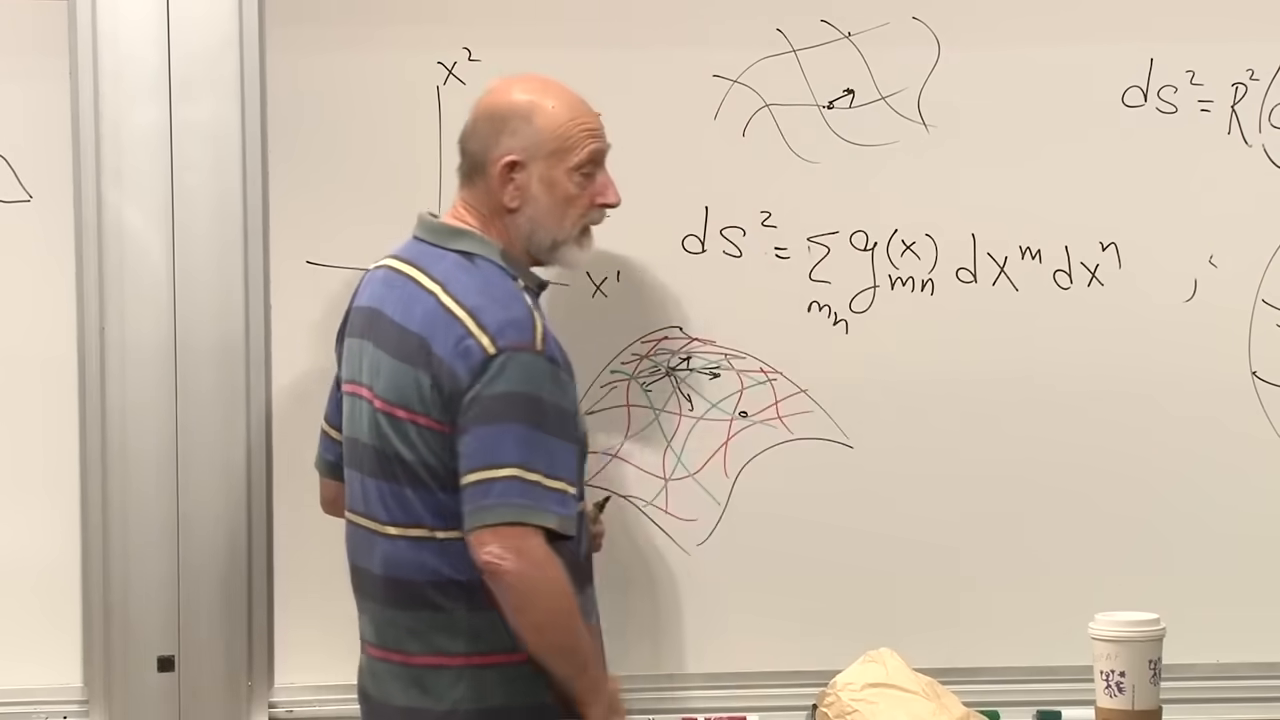
\includegraphics[width=\linewidth]{lecture_01_figure_04.png}
\caption{Una cuadrícula lineal del espacio-tiempo para coordenadas en movimiento uniforme.}
\par\smallskip
\textit{Marco de la clase: 00:19:45.}
\end{figure}

Para la transformación acelerada, una línea de \(z'\) constante satisface
\begin{equation}
 z=z'+\frac12gt^2.
\end{equation}
Es una parábola tumbada. Si prolongamos el movimiento hacia atrás en el tiempo, el ascensor desciende mientras se frena, cambia de sentido y luego acelera hacia arriba. Cada línea vecina de \(z'\) constante es la misma parábola desplazada horizontalmente.

\begin{figure}[H]
\centering
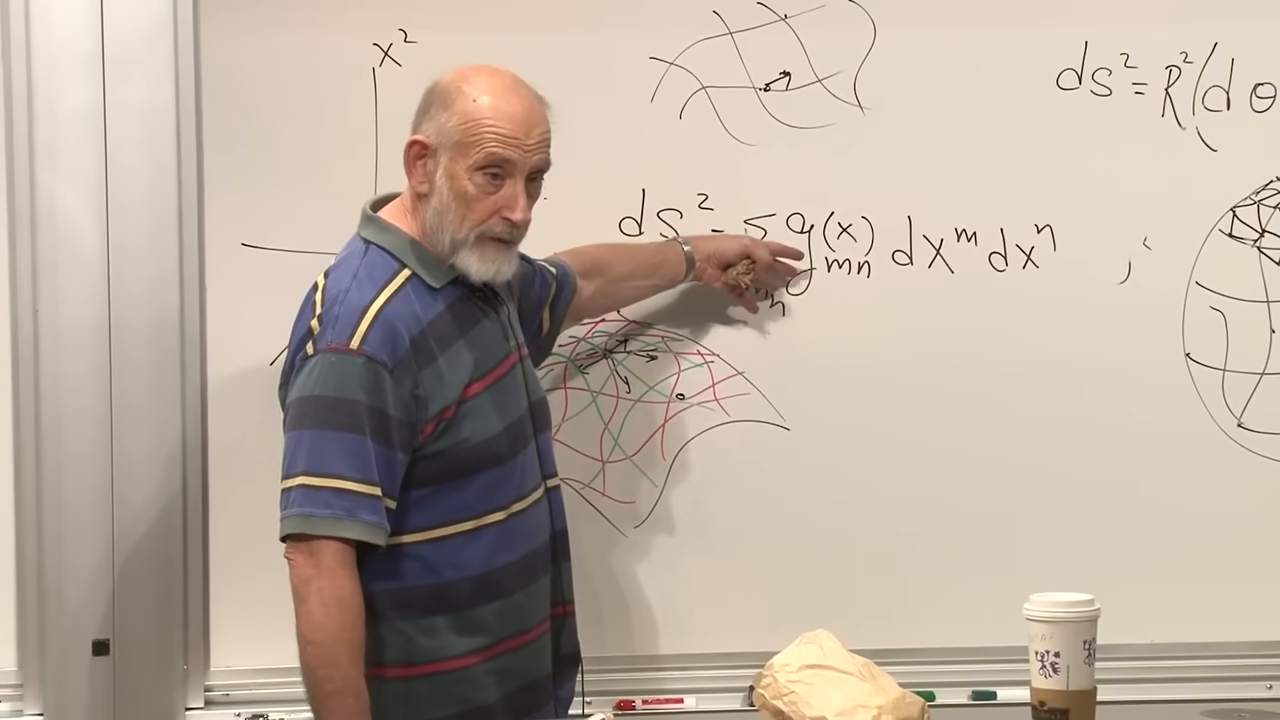
\includegraphics[width=\linewidth]{lecture_01_figure_05.png}
\caption{Curvas de \(z'\) constante para el sistema de coordenadas con aceleración uniforme.}
\par\smallskip
\textit{Marco de la clase: 00:22:25.}
\end{figure}

Esta es la primera pista geométrica. La relatividad especial emplea transformaciones de Lorentz lineales, que llevan líneas rectas del espacio-tiempo a otras líneas rectas. Para representar la aceleración y, por tanto, imitar la gravedad, se necesitan transformaciones curvilíneas de las coordenadas del espacio-tiempo.

Einstein aprovechó este punto, aparentemente modesto, para responder una pregunta nada modesta: ¿afecta la gravedad a la luz? En \(t=0\), hagamos que los sistemas del ascensor y del suelo estén instantáneamente en reposo uno respecto del otro y enviemos un rayo de luz horizontal a través del ascensor. En el sistema no acelerado,
\begin{equation}
 x=ct,\qquad z=0.
\end{equation}
Usando \(z=z'+\tfrac12gt^2\), el mismo rayo en las coordenadas del ascensor satisface
\begin{equation}
 z'=-\frac12gt^2
    =-\frac{g}{2c^2}x^2.
\label{eq:accelerated-light}
\end{equation}
El rayo de luz es recto en el sistema inercial y curvo en el sistema acelerado. Si la aceleración y la gravedad son localmente equivalentes, un campo gravitatorio debe desviar la luz. El argumento establece este efecto antes de que se haya escrito una ecuación de campo para la gravedad.

\begin{figure}[H]
\centering
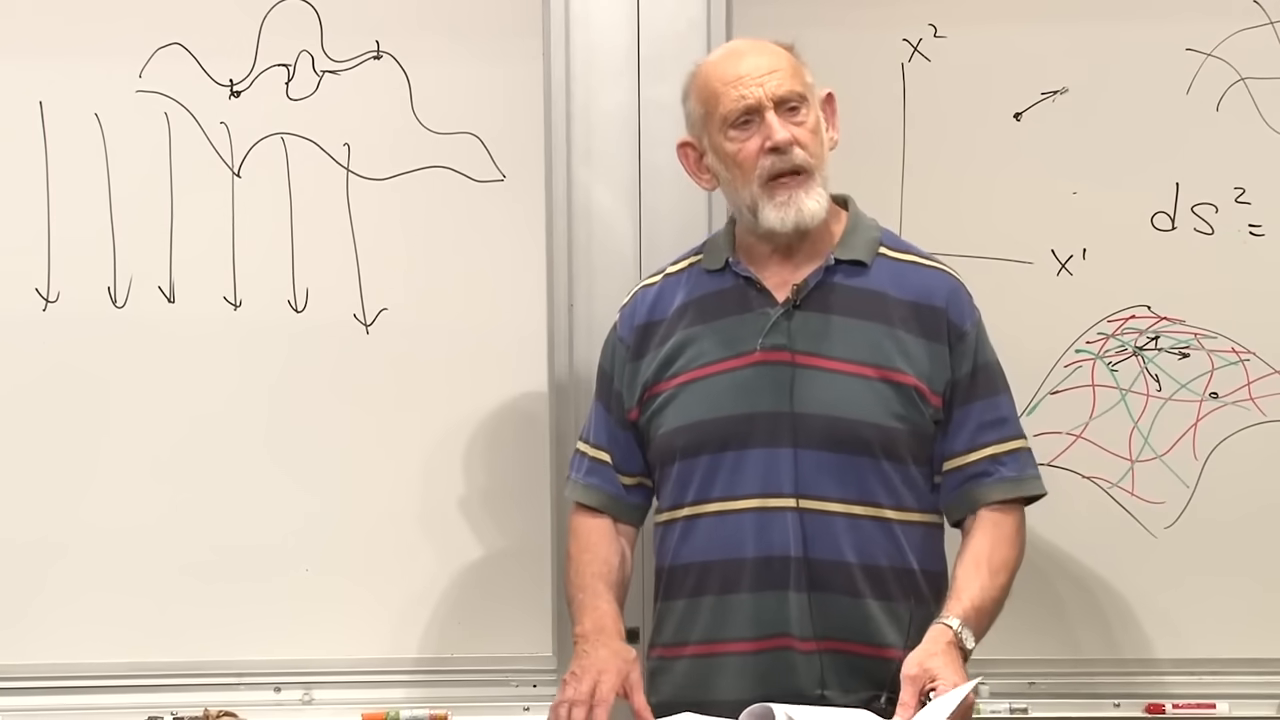
\includegraphics[width=\linewidth]{lecture_01_figure_06.png}
\caption{El rayo de luz horizontal y su trayectoria curva en el sistema acelerado.}
\par\smallskip
\textit{Marco de la clase: 00:28:10.}
\end{figure}

\section{Lo que no puede eliminarse mediante una transformación}

Un sistema acelerado puede generar un campo gravitatorio uniforme aparente. De ello no se sigue que todo campo gravitatorio sea un artefacto de las coordenadas. El campo de una estrella apunta radialmente hacia dentro. Un pequeño laboratorio en caída libre cerca de un punto puede eliminar la aceleración local, pero esa misma transformación no puede eliminar el campo a todos los lados de la estrella.

\begin{figure}[H]
\centering
\includegraphics[width=\linewidth]{lecture_01_figure_07.png}
\caption{Un campo radial y un cuerpo extenso en caída que ponen de manifiesto la aceleración de marea.}
\par\smallskip
\textit{Marco de la clase: 00:32:50.}
\end{figure}

El obstáculo son las fuerzas de marea. Imaginemos a una persona de dos mil millas de altura que cae con los pies por delante. Sus pies están más cerca de la fuente y aceleran más que su cabeza, de modo que se estira. Si se la coloca de lado, las direcciones hacia dentro en lados opuestos tienen componentes que apuntan la una hacia la otra, así que se comprime. En lenguaje newtoniano, puntos vecinos separados por \(\xi^j\) adquieren una aceleración relativa
\begin{equation}
 \delta a^i \simeq \partial_j g^i\,\xi^j.
\label{eq:newtonian-tide}
\end{equation}
Es posible eliminar una aceleración de coordenadas. No se puede eliminar la aceleración relativa entre las partes de un cuerpo extenso en caída libre.

\begin{classroomqa}
\audiencequestion{¿Podrían distintos motores de cohete en la cabeza y en los pies simular el estiramiento y, por tanto, un campo de marea?}
\lecturerresponse{Los motores aplicados ciertamente pueden someter un cuerpo a esfuerzos, pero eso es una fuerza real no gravitatoria que actúa de manera distinta sobre sus partes. Un mero cambio de coordenadas no puede crear una aceleración relativa invariante entre partículas vecinas en caída libre. El diagnóstico se refiere a la caída libre sin fuerzas aplicadas, no a un cuerpo impulsado por cohetes separados.
\lecturetimestamp{00:36:51}}
\end{classroomqa}

Sin embargo, las coordenadas curvas pueden hacer que los campos ficticios parezcan bastante complicados. Un sistema de referencia puede acelerarse verticalmente mientras oscila horizontalmente, lo que produce un campo aparente dependiente del tiempo con ambas componentes. Incluso las coordenadas polares ordinarias ofrecen un ejemplo instructivo. Una partícula libre que se mueve en línea recta cartesiana primero tiene un valor decreciente de \(r(t)\), alcanza un radio mínimo y luego tiene un valor creciente de \(r(t)\). Si alguien solo conociera \(r(t)\) y \(\theta(t)\), podría inferir la existencia de una fuerza repulsiva hacia fuera. En variantes giratorias de estas coordenadas aparecen términos centrífugos y de Coriolis. Son proporcionales a la masa y, por ello, parecen gravitatorios, pero no dejan ninguna deformación de marea invariante en un cuerpo en caída libre.

\begin{classroomqa}
\audiencequestion{¿Qué ocurre si se describe el movimiento con coordenadas angulares o polares?}
\lecturerresponse{La descripción no lineal mediante coordenadas hace que una trayectoria libre recta parezca repelida desde \(r=0\). Esa fuerza centrífuga efectiva es una fuerza de coordenadas. Al volver a un sistema cartesiano inercial, desaparece y no queda ninguna deformación de marea.
\lecturetimestamp{00:37:56}}
\end{classroomqa}

\begin{figure}[H]
\centering
\includegraphics[width=\linewidth]{lecture_01_figure_08.png}
\caption{Descripción en coordenadas polares de una trayectoria recta, con \(r(t)\) y \(\theta(t)\) indicados en la pizarra.}
\par\smallskip
\textit{Marco de la clase: 00:40:20.}
\end{figure}

\begin{classroomqa}
\audiencequestion{¿Pueden varios cuerpos que gravitan cancelarse entre sí y dejar una fuerza de marea nula?}
\lecturerresponse{Las fuerzas pueden cancelarse en un punto elegido, pero la cancelación del valor del campo no cancela, en general, sus derivadas espaciales. Cerca de cualquiera de las fuentes, las trayectorias vecinas siguen adquiriendo aceleraciones distintas. Para que no haya curvatura, el diagnóstico de marea debe anularse en toda la región, no basta con que la fuerza neta se anule en un punto. \lecturetimestamp{00:42:16}}
\end{classroomqa}

\begin{classroomqa}
\audiencequestion{¿Cómo se mide operativamente una fuerza de marea?}
\lecturerresponse{Se deja caer libremente un objeto extenso, como un cristal, y se buscan tensiones y deformaciones que lo estiren en una dirección y lo compriman en otra. Esas deformaciones son medibles y no desaparecen al cambiar las etiquetas de las coordenadas. \lecturetimestamp{00:44:38}}
\end{classroomqa}

\begin{classroomqa}
\audiencequestion{¿Sentiría un efecto radial de marea una persona de dos mil millas de altura en un tiovivo?}
\lecturerresponse{Una persona sujeta al carrusel siente fuerzas de sustentación y, de hecho, podría acabar con dolor de cabeza. El objeto de prueba debe estar en caída libre. Su trayectoria parece complicada en coordenadas giratorias, pero sigue siendo una trayectoria recta sin tensiones en el sistema inercial, así que la fuerza de marea invariante es nula.
\lecturetimestamp{00:45:07}}
\end{classroomqa}

\begin{classroomqa}
\audiencequestion{¿Se puede inclinar el cuerpo en caída para que se cancelen el estiramiento y la compresión?}
\lecturerresponse{Ninguna orientación elimina la deformación completa. El campo radial estira en una dirección principal y comprime en las direcciones transversales. Un cuerpo con extensión finita en todas las direcciones experimenta el patrón completo. \lecturetimestamp{00:47:10}}
\end{classroomqa}

\begin{figure}[H]
\centering
\includegraphics[width=\linewidth]{lecture_01_figure_09.png}
\caption{Estiramiento radial y compresión transversal mostrados conjuntamente para un cuerpo extenso en caída libre.}
\par\smallskip
\textit{Marco de la clase: 00:47:55.}
\end{figure}

\begin{classroomqa}
\audiencequestion{¿Significan las fuerzas de marea que falla el principio de equivalencia?}
\lecturerresponse{Determinan cuán cuidadosamente debe enunciarse. En un sistema lo bastante pequeño como para que el campo gravitatorio varíe de forma despreciable en su interior, la gravedad puede eliminarse, con la precisión pertinente, mediante un sistema de referencia en caída libre. La variación residual a través de un sistema más grande es el campo de marea. \lecturetimestamp{00:48:08}}
\end{classroomqa}

\section{De la geometría de Minkowski a una métrica local}

Ahora nos tomamos un breve descanso de la gravedad. Minkowski ya había enseñado que el espacio-tiempo posee una geometría local invariante. En una dimensión espacial, con \(c=1\),
\begin{equation}
 d\tau^2=dt^2-dx^2.
\label{eq:minkowski-proper-time}
\end{equation}
También se puede definir \(ds^2=dx^2-dt^2=-d\tau^2\). La diferencia es una convención de signatura, no una diferencia física.

\begin{classroomqa}
\audiencequestion{¿Dónde aparece la velocidad de la luz si no se iguala a uno?}
\lecturerresponse{Si \(t\) se mide en unidades de tiempo y \(x\) en unidades de longitud, una forma conveniente es
\(d\tau^2=dt^2-dx^2/c^2\). De manera equivalente, se multiplica por \(c^2\) y se usa
\(c^2d\tau^2=c^2dt^2-dx^2\). Al elegir \(ct\) o \(x/c\) como coordenada, se absorbe el factor de conversión. \lecturetimestamp{00:51:02}}
\end{classroomqa}

\begin{figure}[H]
\centering
\includegraphics[width=\linewidth]{lecture_01_figure_10.png}
\caption{El intervalo de tiempo propio que proporciona el puente geométrico de la relatividad especial a la general.}
\par\smallskip
\textit{Marco de la clase: 00:51:10.}
\end{figure}

Einstein reconoció que el problema de decidir si un campo gravitatorio puede eliminarse se parece a un problema estudiado por Gauss para las superficies y por Riemann en dimensiones arbitrarias: dada una ley local de distancias, ¿cómo se puede decidir si la geometría es realmente curva?

En coordenadas cartesianas euclidianas, el teorema de Pitágoras da
\begin{equation}
 ds^2=(dx^1)^2+(dx^2)^2+\cdots
     =\delta_{mn}\,dx^m dx^n.
\label{eq:euclidean-line-element}
\end{equation}
El rango de los índices es la dimensión del espacio. La notación no cambia si hay dos, tres o veintiséis coordenadas.

\begin{figure}[H]
\centering
\includegraphics[width=\linewidth]{lecture_01_figure_11.png}
\caption{El elemento de línea euclidiano como suma de incrementos de coordenadas al cuadrado.}
\par\smallskip
\textit{Marco de la clase: 00:55:00.}
\end{figure}

Situemos coordenadas arbitrarias \(x^m\) sobre una superficie cualquiera. La distancia entre puntos vecinos viene dada por la forma cuadrática
\begin{equation}
 ds^2=g_{mn}(x)\,dx^m dx^n.
\label{eq:general-line-element}
\end{equation}
Las funciones \(g_{mn}(x)\) son las componentes del tensor métrico. La misma fórmula se aplica también a una superficie plana descrita mediante coordenadas curvilíneas; que las componentes de la métrica no sean constantes no demuestra por sí solo que haya curvatura intrínseca.

\begin{figure}[H]
\centering
\includegraphics[width=\linewidth]{lecture_01_figure_12.png}
\caption{Una forma cuadrática métrica general junto a una red de coordenadas curvilíneas.}
\par\smallskip
\textit{Marco de la clase: 00:58:20.}
\end{figure}

Para una esfera de radio \(R\), cuando \(\theta\) se mide desde un polo,
\begin{equation}
 ds^2=R^2\left(d\theta^2+\sin^2\theta\,d\phi^2\right).
\label{eq:sphere-polar}
\end{equation}
El mismo incremento de longitud cubre una distancia grande cerca del ecuador y pequeña cerca de un polo; la dependencia de la posición que registra el coeficiente es precisamente esa.

\begin{classroomqa}
\audiencequestion{La latitud ordinaria se mide desde el ecuador, así que ¿el coeficiente debería ser un coseno en vez de un seno?}
\lecturerresponse{Sí. Si \(\lambda\) denota la latitud medida desde el ecuador, entonces
\(ds^2=R^2(d\lambda^2+\cos^2\lambda\,d\phi^2)\).
La ecuación \eqref{eq:sphere-polar} emplea el ángulo polar
\(\theta=\pi/2-\lambda\), medido desde el polo norte.
\lecturetimestamp{01:01:03}}
\end{classroomqa}

\begin{figure}[H]
\centering
\includegraphics[width=\linewidth]{lecture_01_figure_13.png}
\caption{La métrica de la esfera y la geometría latitud--longitud que determina su coeficiente dependiente de la posición.}
\par\smallskip
\textit{Marco de la clase: 01:00:30.}
\end{figure}

Las coordenadas más generales pueden introducir términos cruzados \(d\theta\,d\phi\), pero la distancia local sigue siendo cuadrática en los diferenciales. Los términos cúbicos o lineales no forman parte de un elemento de línea riemanniano.

\section{Distancia local y curvatura intrínseca}

\begin{classroomqa}
\audiencequestion{¿La fórmula de la métrica también da la distancia entre dos puntos muy separados?}
\lecturerresponse{No, no mediante una sustitución directa. Da la distancia entre puntos vecinos. Para obtener una distancia macroscópica hace falta una trayectoria e integrar \(ds\); si por distancia se entiende la trayectoria más corta, hay que determinarla a partir de la geometría. Incluso puede haber varias trayectorias localmente más cortas que conecten los mismos extremos. \lecturetimestamp{01:02:30}}
\end{classroomqa}

En una superficie accidentada, imaginemos dos estacas en puntos distantes y una cuerda tensa entre ellas. La cuerda puede rodear una colina por un lado o por el otro, y al mover una colina cambia la ruta que minimiza la longitud. La distancia global depende de la geometría intermedia. La distancia local es más sencilla: la métrica proporciona una pequeña regla en cada punto y la geometría se construye a partir de esas reglas infinitesimales.

\begin{figure}[H]
\centering
\includegraphics[width=\linewidth]{lecture_01_figure_14.png}
\caption{El problema de la distancia global: una ruta tensa debe sortear la superficie entre sus extremos.}
\par\smallskip
\textit{Marco de la clase: 01:04:00.}
\end{figure}

Si las piezas locales pueden colocarse sobre un plano sin estirarlas ni rasgarlas, la geometría intrínseca es plana. No es posible colocar planas todas las piezas cuyas longitudes corresponden a una esfera triangulada y conservar a la vez sus bordes. Por tanto, la métrica plantea un problema preciso: dada \(g_{mn}(x)\), ¿se puede determinar si sus piezas infinitesimales encajan formando un espacio plano?

\begin{figure}[H]
\centering
\includegraphics[width=\linewidth]{lecture_01_figure_15.png}
\caption{La métrica y la carta de coordenadas local interpretadas como piezas infinitesimales a partir de las cuales se construye la geometría.}
\par\smallskip
\textit{Marco de la clase: 01:05:20.}
\end{figure}

\begin{classroomqa}
\audiencequestion{¿Se podría diagnosticar la curvatura midiendo la razón entre la circunferencia y el diámetro?}
\lecturerresponse{Sí, es una prueba útil en dos dimensiones. En una superficie curva, la razón puede diferir de \(\pi\). Sin embargo, en un círculo infinitesimal la desviación aparece en un orden superior, y el método no se generaliza con tanta facilidad como un tensor de curvatura.
\lecturetimestamp{01:07:26}}
\end{classroomqa}

Una región es plana si existe un sistema de coordenadas en el que
\begin{equation}
 g_{mn}=\delta_{mn},
\qquad
 ds^2=\delta_{mn}\,dx^m dx^n
\label{eq:flat-metric}
\end{equation}
en toda esa región. Por tanto, una \(g_{mn}(x)\) complicada puede describir un espacio curvo o simplemente coordenadas curvas en un espacio plano. La cuestión es si una transformación de coordenadas puede eliminar toda la complicación.

\begin{figure}[H]
\centering
\includegraphics[width=\linewidth]{lecture_01_figure_16.png}
\caption{El problema de la métrica formulado en una carta local: ¿se puede transformar su forma curvilínea a la forma plana?}
\par\smallskip
\textit{Marco de la clase: 01:07:15.}
\end{figure}

\begin{classroomqa}
\audiencequestion{¿El elemento de línea esférico supone que cada intervalo pequeño es plano aunque la esfera no lo sea?}
\lecturerresponse{En primer orden, toda superficie suave se aproxima en un punto por su plano tangente. La curvatura se manifiesta en cómo no encajan entre sí las aproximaciones tangentes de puntos vecinos, o en los cambios de orden superior a través de una región finita. Por eso, el comportamiento euclidiano local es compatible con la curvatura global. \lecturetimestamp{01:10:01}}
\end{classroomqa}

\begin{classroomqa}
\audiencequestion{¿Debe ser continua la métrica, y qué ocurre en un pliegue o una grieta?}
\lecturerresponse{La exposición supone que las aplicaciones de coordenadas y la métrica son lo bastante suaves para que existan las derivadas requeridas. Una hoja plegada sin estirarla tiene las mismas distancias intrínsecas a ambos lados del pliegue; su aspecto llamativo es extrínseco. Una geometría realmente singular o no suave requiere un tratamiento aparte y queda fuera del planteamiento suave que se usa aquí. \lecturetimestamp{01:11:25}}
\end{classroomqa}

Esta distinción corresponde a la geometría intrínseca. Doblar una página en el espacio tridimensional cambia su inmersión, pero no las distancias medidas dentro de ella. Una criatura confinada a la página e incapaz de mirar hacia el espacio en el que está inmersa todavía puede medir su geometría intrínseca.

\begin{figure}[H]
\centering
\includegraphics[width=\linewidth]{lecture_01_figure_17.png}
\caption{Una hoja plegada permite distinguir la distancia intrínseca de la apariencia extrínseca.}
\par\smallskip
\textit{Marco de la clase: 01:13:00.}
\end{figure}

\begin{classroomqa}
\audiencequestion{¿Por qué no diagonalizar simplemente la métrica?}
\lecturerresponse{En cualquier punto, una elección adecuada de coordenadas puede diagonalizar la métrica y normalizarla para que adopte la forma plana local. El obstáculo está en hacerlo en toda una región con un único sistema de coordenadas. La curvatura no se puede detectar examinando un solo punto.
\lecturetimestamp{01:13:48}}
\end{classroomqa}

\begin{figure}[H]
\centering
\includegraphics[width=\linewidth]{lecture_01_figure_18.png}
\caption{La métrica cartesiana plana \(\delta_{mn}\) escrita debajo de la forma cuadrática local general.}
\par\smallskip
\textit{Marco de la clase: 01:16:00.}
\end{figure}

Ahora la analogía con la gravedad es exacta, no meramente sugestiva. Una fuerza de coordenadas puede eliminarse, igual que puede eliminarse una descripción curvilínea de un espacio plano. En relatividad general, la aceleración de marea se mide mediante la curvatura. En la notación que veremos más adelante, las líneas de universo vecinas en caída libre satisfacen la ecuación de desviación geodésica
\begin{equation}
 \frac{D^2\xi^\mu}{D\tau^2}
 =-R^\mu{}_{\nu\rho\sigma}
   u^\nu\xi^\rho u^\sigma.
\label{eq:geodesic-deviation-preview}
\end{equation}
Curvatura nula significa que no hay campo de marea invariante; curvatura no nula significa que ninguna elección de coordenadas puede eliminar la gravedad en toda la región.

\section{Dos sistemas de coordenadas y un vector}

Para decidir si una métrica puede transformarse a \(\delta_{mn}\), primero debemos saber cómo se transforman los objetos geométricos. Sean \(x^m\) y \(y^m\) dos sistemas de coordenadas suaves en una misma región:
\begin{equation}
 x^m=x^m(y),\qquad y^m=y^m(x).
\label{eq:mutual-coordinate-maps}
\end{equation}
Los símbolos \(x\) y \(y\) designan sistemas de coordenadas completos, no dos direcciones espaciales particulares.

\begin{figure}[H]
\centering
\includegraphics[width=\linewidth]{lecture_01_figure_19.png}
\caption{Las aplicaciones de coordenadas mutuamente relacionadas \(x^m(y)\) y \(y^m(x)\).}
\par\smallskip
\textit{Marco de la clase: 01:20:35.}
\end{figure}

Para puntos vecinos, la regla de la cadena da
\begin{equation}
 dy^m=\frac{\partial y^m}{\partial x^p}\,dx^p.
\label{eq:differential-transform}
\end{equation}
Se suma sobre el índice repetido \(p\). El desplazamiento en sí es un único vector geométrico; \(dx^p\) y \(dy^m\) son sus componentes en dos sistemas de coordenadas.

\begin{figure}[H]
\centering
\includegraphics[width=\linewidth]{lecture_01_figure_20.png}
\caption{La transformación diferencial de coordenadas obtenida mediante la regla de la cadena.}
\par\smallskip
\textit{Marco de la clase: 01:22:30.}
\end{figure}

\begin{classroomqa}
\audiencequestion{En una cuadrícula curvilínea, ¿qué representan las líneas de coordenadas?}
\lecturerresponse{En dos dimensiones, se obtiene una línea manteniendo fija una coordenada mientras varía la otra. En dimensiones superiores, los conjuntos correspondientes de coordenada constante son hipersuperficies. Sus intersecciones locales definen las direcciones de coordenadas que se usan para descomponer las componentes de los vectores. \lecturetimestamp{01:25:20}}
\end{classroomqa}

Un vector contravariante se define mediante la misma ley de transformación que un desplazamiento de coordenadas:
\begin{equation}
 (V')^m(y)
 =\frac{\partial y^m}{\partial x^p}\,V^p(x).
\label{eq:contravariant-vector}
\end{equation}
La velocidad sobre una superficie es un ejemplo. El vector no cambia al cambiar de coordenadas; sí cambian sus componentes.

\begin{figure}[H]
\centering
\includegraphics[width=\linewidth]{lecture_01_figure_21.png}
\caption{La ley de transformación de un vector contravariante, enmarcada.}
\par\smallskip
\textit{Marco de la clase: 01:29:30.}
\end{figure}

La convención de suma de Einstein omite el signo de sumatorio cuando un índice aparece repetido una vez arriba y otra abajo. Esta convención facilitó la impresión de las fórmulas, pero, aún más importante, hace visible el patrón de contracción.

\begin{classroomqa}
\audiencequestion{¿Se hacen suposiciones especiales sobre los sistemas de coordenadas permitidos?}
\lecturerresponse{Solo se supone que los dos sistemas están relacionados funcionalmente y son lo bastante suaves como para que existan, en la región considerada, las derivadas indicadas y la aplicación inversa. No se supone linealidad ni ortogonalidad. \lecturetimestamp{01:28:12}}
\end{classroomqa}

\section{Covectores y la regla de la cadena}

Sea \(S(x)\) un escalar: tiene un valor bien definido en cada punto, independiente de las etiquetas de las coordenadas. La temperatura y un campo escalar son ejemplos. Las componentes de su gradiente son
\begin{equation}
 W_p=\frac{\partial S}{\partial x^p}.
\label{eq:gradient-covector}
\end{equation}

\begin{figure}[H]
\centering
\includegraphics[width=\linewidth]{lecture_01_figure_22.png}
\caption{Gradiente escalar introducido junto a la ley de transformación contravariante.}
\par\smallskip
\textit{Marco de la clase: 01:31:40.}
\end{figure}

Al aplicar la regla de la cadena en las coordenadas \(y\),
\begin{equation}
 W'_m
 =\frac{\partial S}{\partial y^m}
 =\frac{\partial x^p}{\partial y^m}
  \frac{\partial S}{\partial x^p}
 =\frac{\partial x^p}{\partial y^m}\,W_p.
\label{eq:covariant-vector}
\end{equation}
Esta es la ley de transformación de un vector covariante, o covector. El jacobiano es el inverso del que aparece en
\eqref{eq:contravariant-vector}; por tanto, los índices inferiores y superiores codifican comportamientos de transformación distintos.

\begin{figure}[H]
\centering
\includegraphics[width=\linewidth]{lecture_01_figure_23.png}
\caption{Leyes de transformación contravariante y covariante mostradas juntas.}
\par\smallskip
\textit{Marco de la clase: 01:34:40.}
\end{figure}

\begin{classroomqa}
\audiencequestion{¿Qué relación hay entre los vectores covariantes y los contravariantes?}
\lecturerresponse{En esta etapa se definen como tipos distintos de objetos: los desplazamientos y las velocidades se transforman de una manera, y los gradientes, de la manera inversa. Más adelante, la métrica proporcionará una correspondencia biunívoca que permite bajar o subir un índice. No se debe presuponer esa relación antes de introducir la métrica. \lecturetimestamp{01:37:43}}
\end{classroomqa}

\begin{classroomqa}
\audiencequestion{¿Al bajar un índice, cambiaba antes el signo de la componente temporal?}
\lecturerresponse{Ese signo procedía de la métrica lorentziana. La derivación actual se está realizando primero en geometría euclidiana ordinaria. Para subir o bajar índices siempre se usa la métrica correspondiente; el signo de la componente temporal solo aparece cuando esa métrica tiene signatura lorentziana.
\lecturetimestamp{01:38:29}}
\end{classroomqa}

\begin{classroomqa}
\audiencequestion{¿Deberíamos considerar ya las dos leyes de transformación como dos descripciones en componentes del mismo vector?}
\lecturerresponse{Todavía no. Una vez que se dispone de la métrica, un vector contravariante \(V^m\) puede convertirse en un covector \(V_m=g_{mn}V^n\). Hasta establecer esa correspondencia, los objetos con índices superiores e inferiores son lógicamente distintos. \lecturetimestamp{01:39:00}}
\end{classroomqa}

Estas fórmulas son independientes de la dimensión. Cambia el rango de los índices, pero no las leyes de transformación.

\section{Tensores con más de un índice}

Consideremos dos vectores contravariantes \(V^m\) y \(U^n\). Su producto
\begin{equation}
 T^{mn}=V^mU^n
\label{eq:rank-two-product}
\end{equation}
es un tensor contravariante de rango dos. En tres dimensiones tiene nueve componentes; en cuatro dimensiones, dieciséis. El orden de los índices importa, salvo que se especifique una simetría: \(T^{mn}\) no tiene por qué ser igual a \(T^{nm}\).

\begin{figure}[H]
\centering
\includegraphics[width=\linewidth]{lecture_01_figure_24.png}
\caption{Un tensor de rango dos construido como el producto de dos vectores contravariantes.}
\par\smallskip
\textit{Fotograma de la clase: 01:43:40.}
\end{figure}

Cada índice superior aporta un jacobiano directo:
\begin{equation}
 (T')^{mn}
 =\frac{\partial y^m}{\partial x^p}
  \frac{\partial y^n}{\partial x^q}
  T^{pq}.
\label{eq:rank-two-contravariant}
\end{equation}
La construcción mediante el producto motiva esta regla, pero la ley de transformación es lo que define un tensor. Un tensor contravariante de rango tres tendría tres factores jacobianos de este tipo.

\begin{figure}[H]
\centering
\includegraphics[width=\linewidth]{lecture_01_figure_25.png}
\caption{Los dos factores jacobianos en la transformación de \(T^{mn}\).}
\par\smallskip
\textit{Fotograma de la clase: 01:44:20.}
\end{figure}

Del mismo modo, cada índice inferior aporta un jacobiano inverso:
\begin{equation}
 T'_{mn}
 =\frac{\partial x^p}{\partial y^m}
  \frac{\partial x^q}{\partial y^n}
  T_{pq}.
\label{eq:rank-two-covariant}
\end{equation}
Un tensor mixto utiliza un factor de cada tipo.

\begin{figure}[H]
\centering
\includegraphics[width=\linewidth]{lecture_01_figure_26.png}
\caption{La ley de transformación completa para un tensor con dos índices covariantes.}
\par\smallskip
\textit{Fotograma de la clase: 01:47:30.}
\end{figure}

El mismo formalismo de transformación se aplica ahora a la métrica. Como el intervalo es un escalar, debe tener el mismo valor en ambos sistemas de coordenadas:
\begin{align}
 ds^2
 &=g_{mn}(x)\,dx^m dx^n,\\
 dx^m
 &=\frac{\partial x^m}{\partial y^p}\,dy^p.
\end{align}
La sustitución completa la expresión que quedó sin terminar en la pizarra:
\begin{equation}
 g'_{pq}(y)
 =\frac{\partial x^m}{\partial y^p}
  \frac{\partial x^n}{\partial y^q}
  g_{mn}(x(y)).
\label{eq:l1-metric-transformation}
\end{equation}
Así pues, \(g_{mn}\) es un tensor covariante de rango dos.

\begin{figure}[H]
\centering
\includegraphics[width=\linewidth]{lecture_01_figure_27.png}
\caption{La transformación de la métrica, iniciada a partir de la invariancia del elemento de línea al final de la clase.}
\par\smallskip
\textit{Fotograma de la clase: 01:48:40.}
\end{figure}

La pregunta física inicial se ha convertido ahora en una pregunta matemática. Dada \(g_{mn}(x)\), ¿existe una transformación de coordenadas para la cual \(g'_{mn}=\delta_{mn}\) en toda la región? Si es así, la complejidad aparente se debe solo a las coordenadas. Si no, el obstáculo es la curvatura y, en el espacio-tiempo, ese obstáculo constituye el contenido invariante de la gravedad.